\documentclass{beamer}
\usetheme[sectionpage=none, progressbar=frametitle,background=light]{metropolis}

\usepackage[english]{babel}

\usepackage{graphics}
\usepackage{appendixnumberbeamer}

\usepackage{algorithm2e}
\usepackage{amssymb,amsmath,amsthm, bm}
\usepackage{subcaption}
\usepackage{tikz, enumitem}
\usepackage{tabularx}

\usetikzlibrary{positioning}

%General declarations
\DeclareMathOperator{\Ima}{Im}
\DeclareMathOperator{\Ker}{Ker}
\DeclareMathOperator{\low}{low}
\DeclareMathOperator*{\argmin}{arg\,min}
\DeclareMathOperator*{\argmax}{arg\,max}

\newcommand{\R}{\mathbb{R}}
\newcommand{\Q}{\mathbb{Q}}
\newcommand{\Z}{\mathbb{Z}}
\newcommand{\F}{\mathbb{F}}
\newcommand{\N}{\mathbb{N}}
\newcommand{\Sphere}{\mathbb{S}}
\newcommand{\BigO}{\mathcal{O}}

\newcommand{\defunder}[1]{\underset{\text{def.}}{#1} \:}
\newcommand{\vspan}{\operatorname{span}}

\newcommand{\LexicographicOrderChain}{\sqsubseteq_{lex}}
\newcommand{\LexicographicStrictOrderChain}{\sqsubset_{lex}}
\newcommand{\LexicographicOrderEdgeSets}{\sqsubseteq_{\ee}}

\newcommand{\GraphV}{\mathcal{V}}
\newcommand{\GraphE}{\mathcal{E}}

\newcommand{\VKer}{V^{\Ker}}
\newcommand{\nKer}{n^{\Ker}}

% Lexicographic order
\newcommand{\seb}{\mathbf{SEB}}
\newcommand{\circumcenter}[1]{\operatorname{C_C}\left({#1}\right)}

\newcommand{\rseb}{\operatorname{R_B}}
\newcommand{\circrad}{\operatorname{R_C}}
\newcommand{\TOrderSimplex}{\leq_\infty}
\newcommand{\TOrderSimplexStrict}{<_\infty}
\newcommand{\TReverseOrderSimplexStrict}{>_\infty}
\newcommand{\lift}{\operatorname{lift}}
\newcommand{\Krad}[1]{\mu_{#1}}
\newcommand{\WDist}{\operatorname{D}}

\newcommand{\SOrderChain}{\sqsubseteq_\infty}
\newcommand{\SOrderChainStrict}{\sqsubset_\infty}
\newcommand{\norm}[1]{\left\lVert #1 \right\rVert}
\newcommand{\CH}{\mathcal{CH}}

\newcommand{\Cchains}{\mathbf{C}}
\newcommand{\Zchains}{\mathbf{Z}}
\newcommand{\Bchains}{\mathbf{B}}
\newcommand{\Homol}{\mathcal{H}}
\newcommand{\HomolP}{\mathcal{H}^{pers.}}

\newcommand{\CritBasis}{\mathbf{b}}
\newcommand{\Crit}{\operatorname{crit}}
\newcommand{\ZchainMin}{\Zchains^{\min}}

\newcommand{\ee}{\mathbf{e}}
\newcommand{\Delaunay}{\mathcal{D}el}
\newcommand{\Link}[1]{\operatorname{lk}_{#1}}
\newcommand{\LLink}[1]{\operatorname{llk}_{#1}}
\newcommand{\LinkDel}{\Link{\Delaunay(\mathbf{P})}}
\newcommand{\LLinkDel}{\LLink{\Delaunay(\mathbf{P})}}

\newcommand{\Ack}{\bm{\alpha}}

\newcommand{\Vspan}{\operatorname{span}}
\newcommand{\Mlex}{M_{lex}}

\setbeamerfont{footnote}{size=\fontsize{5pt}{5pt}\selectfont}
\setbeamerfont{footnote mark}{size=\fontsize{5pt}{5pt}\selectfont}

\title{Planimetric simplification and lexicographic optimal chains for 3D urban scene reconstruction}
\author[Julien Vuillamy]{Julien Vuillamy}
\institute[]{Dassault Systèmes Provence - INRIA Sophia Antipolis TITANE}
\date{September 17, 2021}
\titlegraphic{
	\vspace{7cm}\flushright\centering
	\includegraphics[width=0.25\linewidth]{front/logo-ds}\hspace{1cm}
	\includegraphics[width=0.25\linewidth]{front/logo-anrt}\hspace{1cm}
	\includegraphics[width=0.25\linewidth]{front/logo-inria}
}

\graphicspath{{images}}

\setcounter{tocdepth}{1}
	
\begin{document}
	\begin{frame}
		\titlepage
	\end{frame}
		
%	\section*{Outline}
	\begin{frame}{Outline}
% 	    \tableofcontents
	\end{frame}
	
	\section{Introduction}

\begin{frame}{Representations of urban spaces}
	\centering
	\scriptsize
	\pause
	\begin{minipage}{0.5\linewidth}
		\centering
		\includegraphics[width=0.9\linewidth]{context/maps}\\
		2D maps
	\end{minipage}%
	\pause%
	\begin{minipage}{0.5\linewidth}
		\centering
		\includegraphics[width=0.9\linewidth]{context/dense_visu}\\
		3D visualization
	\end{minipage}%
	\pause
	
	\begin{minipage}{0.5\linewidth}
		\centering
		\includegraphics[width=0.9\linewidth]{context/lods}\\
		Geographic Information Systems (GIS)
	\end{minipage}%
	\pause%
	\begin{minipage}{0.5\linewidth}
		\centering
		\includegraphics[width=0.9\linewidth]{context/bim}\\
		Building information model (BIM)
	\end{minipage}
\end{frame}

\begin{frame}[t]{Why do we need 3D models?}
	\textbf{Visualization}
	\vfill
	\begin{figure}
		\centering
		\begin{subfigure}[t]{0.45\linewidth}
			\includegraphics[width=\linewidth]{context/dense_visu}
			\subcaption*{Dense mesh representation \footnote[frame]{Google Maps}}
		\end{subfigure}
		\hfill%
		\begin{subfigure}[t]{0.45\linewidth}
			\includegraphics[width=\linewidth]{context/lod_visu}
			\subcaption*{LOD1 visualization \footnote[frame]{Bien'ici}}
		\end{subfigure}
	\end{figure}
\end{frame}

\begin{frame}[t]{Why do we need 3D models?}
	\textbf{Simulation}
	\vfill
	\begin{figure}
		\centering
		\begin{subfigure}[t]{0.45\linewidth}
			\includegraphics[width=\linewidth]{context/simulation_wind}
			\subcaption*{Wind simulation \footnote[frame]{SIMULIA, Dassault Systèmes}}
		\end{subfigure}
		\hfill%
		\begin{subfigure}[t]{0.45\linewidth}
			\includegraphics[width=\linewidth]{context/simulation_lineofsight}
			\subcaption*{5G connectivity \footnote[frame]{SIRADEL}}
		\end{subfigure}
	\end{figure}
\end{frame}

\begin{frame}[t]{Why do we need 3D models?}
	\textbf{Change tracking}
	\vfill
	\begin{figure}
		\centering
		\begin{subfigure}[t]{0.45\linewidth}
			\includegraphics[width=\linewidth]{context/lod_diff_v2}
			\subcaption*{Permit verification \footnote[frame]{Taken from \cite{biljecki_EffectAcquisition_2018}}}
		\end{subfigure}%
		\hfill%
		\begin{subfigure}[t]{0.45\linewidth}
			\includegraphics[width=\linewidth]{context/building_inspection}
			\subcaption*{Building inspection \footnote[frame]{\href{https://www.engineering.com/story/automating-facility-inspection-with-drones}{Engineering.com \ExternalLink}}}
		\end{subfigure}
	\end{figure}	
\end{frame}

\begin{frame}{Acquisitions}
	\small
	\centering
	\begin{minipage}{0.5\linewidth}
		\centering
		\textbf{LiDAR technologies}
	\end{minipage}%
	\begin{minipage}{0.5\linewidth}
		\centering
		\textbf{Photogrammetry}
	\end{minipage}

	\begin{minipage}{0.5\linewidth}
		\centering
		\includegraphics[width=0.7\linewidth]{context/lidar_method}			
	\end{minipage}%
	\begin{minipage}{0.5\linewidth}
		\centering
		\includegraphics[width=0.7\linewidth]{context/photo_method}
	\end{minipage}

	\begin{minipage}{0.5\linewidth}
		\centering
		\includegraphics[width=0.8\linewidth]{context/lidar}	
	\end{minipage}%
	\begin{minipage}{0.5\linewidth}
		\centering
		\includegraphics[width=0.8\linewidth]{context/photogrammetry}	
	\end{minipage}%
	
	\blfootnote{Images from \href{https://wingtra.com/drone-photogrammetry-vs-lidar}{Wingtra \ExternalLink}}
\end{frame}

\begin{frame}{Scope of interest}
	\textbf{Inputs:} Point clouds (LiDAR or Photogrammetry) \\
	\textbf{Semi-automatic} methods \\
	\pause
	
	\vspace{0.5cm}
	
	\begin{tabular}{ll}
		\textbf{Parsimonious representation} & \textbf{Dense representation} \\
		LOD2 reconstruction & Triangular mesh \\
		Buildings & Any urban object \\
		Strong regularity priors & No priors \\
	\end{tabular}
\end{frame}
	\section{Parsimonious representations from 2D partitions}
\begin{frame}{Reconstruction pipeline}
	
\end{frame}

\begin{frame}
\end{frame}

\begin{frame}
\end{frame}

	\section{Dense representations from lexicographic optimal chains}

\graphicspath{{images/lexicographic}}

% Intuition
\begin{frame}[t]{Intuition}
	\centering
	\newcommand{\legendsize}{6pt}
	\tikzset{legend/.style = {rectangle, text width=0.2\linewidth}}
	\begin{tikzpicture}
		\onslide<1>{
			\node (pointcloud)
			{\includegraphics[width=0.8\linewidth]{intuition/state_0}};
		}
		\onslide<2>{
			\node (pointcloud)
			{\includegraphics[width=0.8\linewidth]{intuition/state_1}};
		}
		\onslide<3>{
			\node (pointcloud)
			{\includegraphics[width=0.8\linewidth]{intuition/state_2}};
		}
		\onslide<4>{
			\node (pointcloud)
			{\includegraphics[width=0.8\linewidth]{intuition/state_3}};
		}
		\node[legend, anchor=south east] at (pointcloud.south east){
			\fontsize{\legendsize}{9pt}\selectfont
			\begin{itemize}[itemsep=0pt,partopsep=0pt,topsep=0pt]
				\item[{\includegraphics[width=\legendsize]{intuition/inlier}}]{Inlier}
				\item[{\includegraphics[width=\legendsize]{intuition/endpoint}}]{Endpoint}
				\item[{
\includegraphics[width=\legendsize]{intuition/outlier}}]{Outlier}
			\end{itemize}
		};
	\end{tikzpicture}
		
	\begin{center}
		\small
		\only<2>{
		\begin{equation*}
			\min_P \sum_{e \in P} \operatorname{length}(e)
		\end{equation*}
		}
		\only<3>{
		\begin{equation*}
			\min_P \sum_{e \in P} \operatorname{length}(e)^2
		\end{equation*}
		}
		\only<4>{
		\begin{equation*}
			\min_P \sum_{e \in P} \operatorname{length}(e)^p
		\end{equation*}
		}
	\end{center}
\end{frame}

% Crash course
\begin{frame}{Simplicial homology}
	\centering
	\begin{tabular}{ll}
		Simplices & \raisebox{-.5\height}{\includegraphics[width=0.5\textwidth]{course/simplices}}
	\end{tabular}
	
	\begin{tabular}{ll} 
		Simplicial complex & \raisebox{-.5\height}{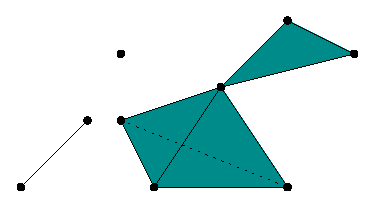
\includegraphics[width=0.4\textwidth]{course/complex}}
	\end{tabular}
	
	A \textbf{\textit{k}-chain} $A$ with coefficients in $\F$ is a formal sum of $k$-simplices:
	\begin{equation*}
		A = \sum_{i} x_i \sigma_i, \text{ with } x_i \in \F \; \text{and} \;\sigma_i \in K^{(k)}
	\end{equation*}
\end{frame}

\begin{frame}{Boundary operator}
	The \textbf{boundary operator} $\partial_k : \Cchains_{k}(K) \to \Cchains_{k-1}(K)$ is the linear map defined for any $k$-simplex $\sigma = [a_0, \dots, a_k]$ as:
	\[
	\partial_k \sigma  \defunder{=}\sum_{i=0}^{k} (-1)^{i} [a_0,\dots, \widehat{a_i},\dots, a_k]
	\]
	
	\begin{center}
		\includegraphics[width=0.8\textwidth]{course/boundary}
	\end{center}
\end{frame}

\begin{frame}{Cycles \& Boundaries}
	The kernels and images of the boundary operator form respectively the vector space of \textbf{cycles} and \textbf{boundaries}:
	\begin{align*}
		\Zchains_{k}(K) &\defunder{=} \Ker \partial_k = \Big\{ \Gamma \in \Cchains_{k}(K), \partial_k \Gamma = 0 \Big\} 
		%\label{definition:absolute-cycles}
		\\
		\Bchains_k(K) &\defunder{=} \Ima \partial_{k+1} = \Big\{ \Gamma \in \Cchains_{k}(K), \exists A \in \Cchains_{k+1}(K) \mid \Gamma = \partial_{k+1} A \Big\} 
		%\label{definition:absolute-boundaries}
	\end{align*}
\end{frame}

\begin{frame}{Boundaries have no boundaries}
	Fundamental property
	\begin{tabular}{ll}
	$\partial_{k} \partial_{k+1} = 0$ & "Boundaries have no boundaries" \\
	\pause
	$\Bchains_k(K) \subset \Zchains_k(K)$ & "All boundaries are cycles"
	\end{tabular}

	\pause
	\begin{center}
		\includegraphics[width=\textwidth]{course/sequence}
	\end{center}
\end{frame}


% Codimension 1: Algorithm
\begin{frame}
	\begin{minipage}[t][0.5\textheight][t]{0.8\linewidth}
		\scriptsize
		\begin{algorithm}[H]
			%			\caption{Lexicographic min-cut}\label{algorithm:Lex-OHCP}
			\SetKwInOut{Input}{Inputs}
			\SetKwInOut{Output}{Output}
			\SetKw{Continue}{continue}
			\SetKw{Or}{or}
			\Input{$G = (\GraphV, \GraphE)$ and $\alpha_1, \alpha_2 \in \GraphV$, with $\GraphE=\{e_i,i=1,\dots,n\}$ in decreasing order}
			\Output{$\Gamma_{\operatorname{LMC}}$}
			\alert<+>{$\Gamma_{\operatorname{LMC}} \leftarrow \varnothing$} \\
			\alert<+>{\For{$v \in \GraphV$} {
					\textbf{MakeSet}(v)
			}}
			
			\For{$e \in \GraphE$ in decreasing order}{
				\alert<+>{$e = (v_1, v_2) \in \GraphV\times \GraphV$} \\
				\alert<+>{$r_1 \leftarrow \textbf{FindSet}(v_1)$, $r_2 \leftarrow \textbf{FindSet}(v_2)$ \\
					$c_1 \leftarrow \textbf{FindSet}(\alpha_1)$, $c_2 \leftarrow \textbf{FindSet}(\alpha_2)$} \\
				\eIf{\alert<+>{$\{ r_1, r_2\} = \{ c_1, c_2 \}$}}{
					$\Gamma_{\operatorname{LMC}} \leftarrow \Gamma_{\operatorname{LMC}} \cup e$
				}
				{
					$\textbf{UnionSet}(r_1, r_2)$
				}
			}
		\end{algorithm}
	\end{minipage}		
\end{frame}
	\section{Conclusion}
\begin{frame}{Conclusion (I)}
\small
\textbf{Parsimonious representations}
\begin{itemize}
	\item<+-> Reconstruction pipeline for LOD2 reconstruction.
	\item<+-> Defining fidelity and regularity terms based on line movement.
	\item<+-> Using Riemannian gradient descent algorithm
\end{itemize}
	
\textbf{Continuation}
\begin{itemize}
	\item Improve the coherence between 2D simplification and 3D data.
	\item Iterative version between detection, simplification and consolidation parts.
	\item Simplification process on 3D polyhedral arrangements.
\end{itemize}

\end{frame}

\begin{frame}{Conclusion (II)}
\small
\textbf{Dense representations}
\begin{itemize}
	\item<+-> Total order on simplices;
	\item<+-> General algorithms based on matrix reduction for persistent homology;
	\item<+-> Efficient versions for closed surface and open surface reconstruction given its boundary;
	\item<+-> Critical basis and application using a sharp edge detector for automatic surface reconstruction.
\end{itemize}

\textbf{Continuation}
\begin{itemize}
	\item Persistent version of algorithms
	\item Automatic interior/exterior detection
	\item Weighted points and regular triangulations	
\end{itemize}

\end{frame}

\begin{frame}[standout]
	Thank you!
\end{frame}
		
	\appendix
	
	\graphicspath{{images/appendices}}

\section*{Appendices}

\begin{frame}{Variational formulation of Delaunay triangulations (I)}
	\scriptsize 
	\begin{minipage}{0.3\linewidth}
		\centering
		\includegraphics[width=\linewidth]{height_difference}
	\end{minipage}%
	\hfill%
	\begin{minipage}{0.65\linewidth}
		\textbf{Variational characterization} of Delaunay triangulation \cite{musin_ConstructionVoronoiDiagram_2003, chen_OptimalDelaunayTriangulations_2004}
		
		\[
		\begin{aligned}
			f_\sigma : |\sigma| &\to \R\\
			x  &\mapsto f_\sigma(x) \defunder{=} \sum_i \lambda_i(x) \norm{P_i}^2 - \norm{x}^2
		\end{aligned}
		\]
		
		\[
		w_p(\sigma) \defunder{=} \| f_\sigma \|_{p} =  \left(  \int_{|\sigma|} f_\sigma(x)^p dx \right)^{\frac{1}{p}}
		\]
		
		\[
		\Delaunay(\mathbf{P}) = \argmin_{\mathcal{T} \in \mathcal{V}_{\mathbf{P}}} \left(\sum_{\sigma \in \mathcal{T}} w_p(\sigma)^p \right)^{\frac{1}{p}}
		\] where $\mathcal{V}_{\mathbf{P}}$ : set of all triangulations of the convex hull $\CH(\mathbf{P})$.
	\end{minipage}
\end{frame}

\begin{frame}{Variational formulation of Delaunay triangulations (II)}
	\scriptsize

	Equivalent formulation in terms of chains
	\[
		\begin{aligned}
			\norm { \Gamma }_{(p)} : \Cchains_d(K_{\mathbf{P}}) &\to \R\\
			\Gamma &\mapsto \sum_{\sigma \in K^{(d)}} | \Gamma( \sigma)|  w_p(\sigma)^p	
		\end{aligned}
	\]
	
	\begin{block}{\scriptsize Variational formulation (simplicial chains)}
	Denote by $\beta_{\mathbf{P}} \in \Bchains_{d-1}(K_{\mathbf{P}})$ the $(d-1)$-boundary made of the simplices belonging to the boundary of $\mathcal{CH}(\mathbf{P})$. For any $p\in [1, \infty)$, define the chain
	\begin{equation*}
		\Gamma_{\min} \defunder{=} \argmin_{\substack{\Gamma \in \Cchains_{d}(K_{\mathbf{P}})\\
				\partial \Gamma = \beta_{\mathbf{P}}}} \norm{\Gamma}_{(p)}
	\end{equation*}
	The support $|\Gamma_{\min}|$ of $\Gamma_{\min}$ corresponds to all $d$-simplices of the Delaunay triangulation of $\mathbf{P}$.
	\end{block}
\end{frame}

\begin{frame}{Generalizing the total order (I)}
	
\scriptsize
\begin{block}{\scriptsize Weighted distance}
Given two weighted points $(P_1,\mu_1), (P_2,\mu_2) \in \R^d\times \R$ their weighted distance is defined as:
\[
\WDist \left( (P_1,\mu_1), (P_2,\mu_2) \right) \defunder{=} (P_1-P_2)^2 - \mu_1 - \mu_2 
\]
\end{block}

\textbf{Circumweight} (Generalized circumscribed sphere radius)
\[
	\mu_C\left(\sigma \right)  \defunder{=} \min \left\{ \mu \in \R, \exists P \in \R^d, \forall (P_i,\mu_i) \in \sigma, \: \WDist \left(  (P, \mu), (P_i, \mu_i) \right) = 0 \right\}
\]

\textbf{Bounding weight} (Generalized smallest enclosing ball radius)
\[
	\mu_B\left(\sigma \right)  \defunder{=} \min \left\{ \mu \in \R, \exists P \in \R^d, \forall (P_i,\mu_i) \in \sigma, \: \WDist \left(  (P, \mu), (P_i, \mu_i) \right) \leq 0 \right\}
\]

\end{frame}

\begin{frame}{Generalizing the total order (II)}
	\scriptsize
	
	\begin{minipage}{0.6\linewidth}
		\textbf{Minimal face} $\Theta(\sigma)$ verifying: $\mu_B(\Theta(\sigma)) = \mu_B(\sigma)$
		
		\textbf{Sequence of inclusion-increasing faces}
		\begin{eqnarray*}
			\Theta_0(\sigma) & \defunder{=} & \Theta(\sigma) \\
			\Theta_k(\sigma) & \defunder{=} & \argmin_{\substack{\Theta_{k-1}(\sigma) \preceq \tau 	\preceq \sigma\\ \dim{\tau} = \dim{\Theta_{k-1}(\sigma) + 1}}} \mu_C(\tau) \\
			\mu_k(\sigma) &\defunder{=}& \mu_C(\Theta_{k}(\sigma))
		\end{eqnarray*}
	\end{minipage}%
	\begin{minipage}{0.4\linewidth}
		\centering
		\includegraphics[width=0.95\linewidth]{theta_for_tetra}
	\end{minipage}

	\begin{block}{\scriptsize Generalized total order on $k$-simplices} For $\sigma_1, \sigma_2 \in K^{(d)}$, \[
			\sigma_1 \leq \sigma_2  
			\defunder{\iff}
			\sigma_1 = \sigma_2 \quad \operatorname{or} \quad
			\begin{cases}
				\Krad{0}(\sigma_1) < \Krad{0}(\sigma_2) &\\
				\quad \operatorname{or} &\\
				\exists k\geq 1, \: \Krad{k}(\sigma_1) > \Krad{k}(\sigma_2) &\\ 
				\operatorname{and} \: \forall j, \: 0\leq j < k, \: \Krad{j}(\sigma_1) = \Krad{j}(\sigma_2) &
			\end{cases}
		\]
	\end{block}
\end{frame}

\begin{frame}{Generalizing the total order (III)}
\scriptsize
\begin{theorem}
	Let $\mathbf{P} = \{(P_1, \mu_1) , \ldots, (P_N, \mu_N) \} \subset \R^d \times \R$, with $N \geq d+1$ be in general position and let $K_{\mathbf{P}}$ be the $d$-dimensional full complex  over $\mathbf{P}$. Denote by $\beta_{\mathbf{P}} \in \Bchains_{d-1}(K_{\mathbf{P}})$ the $(d-1)$-boundary made of simplices belonging to the boundary of $\mathcal{CH}(\mathbf{P})$. Define the chain
	\begin{equation*}
		\Gamma_{\min} \defunder{=}  \min_{\LexicographicOrderChain}  \{ \Gamma \in  \Cchains_d(K_{\mathbf{P}}),  \partial \Gamma = \beta_{\mathbf{P}} \}
	\end{equation*}
	The support $|\Gamma_{\min}|$ of  $\Gamma_{\min}$ corresponds to the $d$-simplices of the regular triangulation of $\mathbf{P}$.
\end{theorem}

\end{frame}

%\begin{frame}{Non-manifold configurations}
%\includegraphics[width=0.5\linewidth]{nonmanifold1}%
%\includegraphics[width=0.5\linewidth]{nonmanifold2}%
%\end{frame}

\begin{frame}{Comparison with other methods}
	\scriptsize
	
	\begin{minipage}{0.5\linewidth}
		\centering
		\includegraphics[width=0.95\linewidth]{closed_points}		
		Input set of points
	\end{minipage}%
	\hfill
	\begin{minipage}{0.5\linewidth}
		\centering
		\includegraphics[width=0.95\linewidth]{closed_lex}	
		Lexicographic optimal cycle
	\end{minipage}
	
	\begin{minipage}{0.5\linewidth}
		\centering
		\includegraphics[width=0.95\linewidth]{closed_poisson}	
		Poisson reconstruction
	\end{minipage}%
	\begin{minipage}{0.5\linewidth}
		\centering
		\includegraphics[width=0.95\linewidth]{closed_scalespace}	
		Advancing front reconstruction
	\end{minipage}
\end{frame}

\begin{frame}{Influence of topological information}
	\scriptsize
	\includegraphics[width=\linewidth]{discovering_handle}
	\begin{tabularx}{\linewidth}{@{}YYY@{}}
		Global lexicographic cut & Single set of constraints & Additional constraints
	\end{tabularx}
\end{frame}

\begin{frame}{Theoretical guarantees}
	\scriptsize
	For a Čech or Vietoris-Rips complex, under very strict conditions linking the point set sampling, the parameter of the complex and the reach of the underlying manifold of Euclidean space, the minimal lexicographic chain in the fundamental class of the complex using the described simplex order is a triangulation of the sampled manifold \cite{cohen-steiner_LexicographicOptimalChains_2019}.
	
	\includegraphics[width=\linewidth]{torus_3}	
\end{frame}

\begin{frame}{Spatial decomposition}
	\textbf{Tiling strategy} for large point clouds
	\begin{center}
		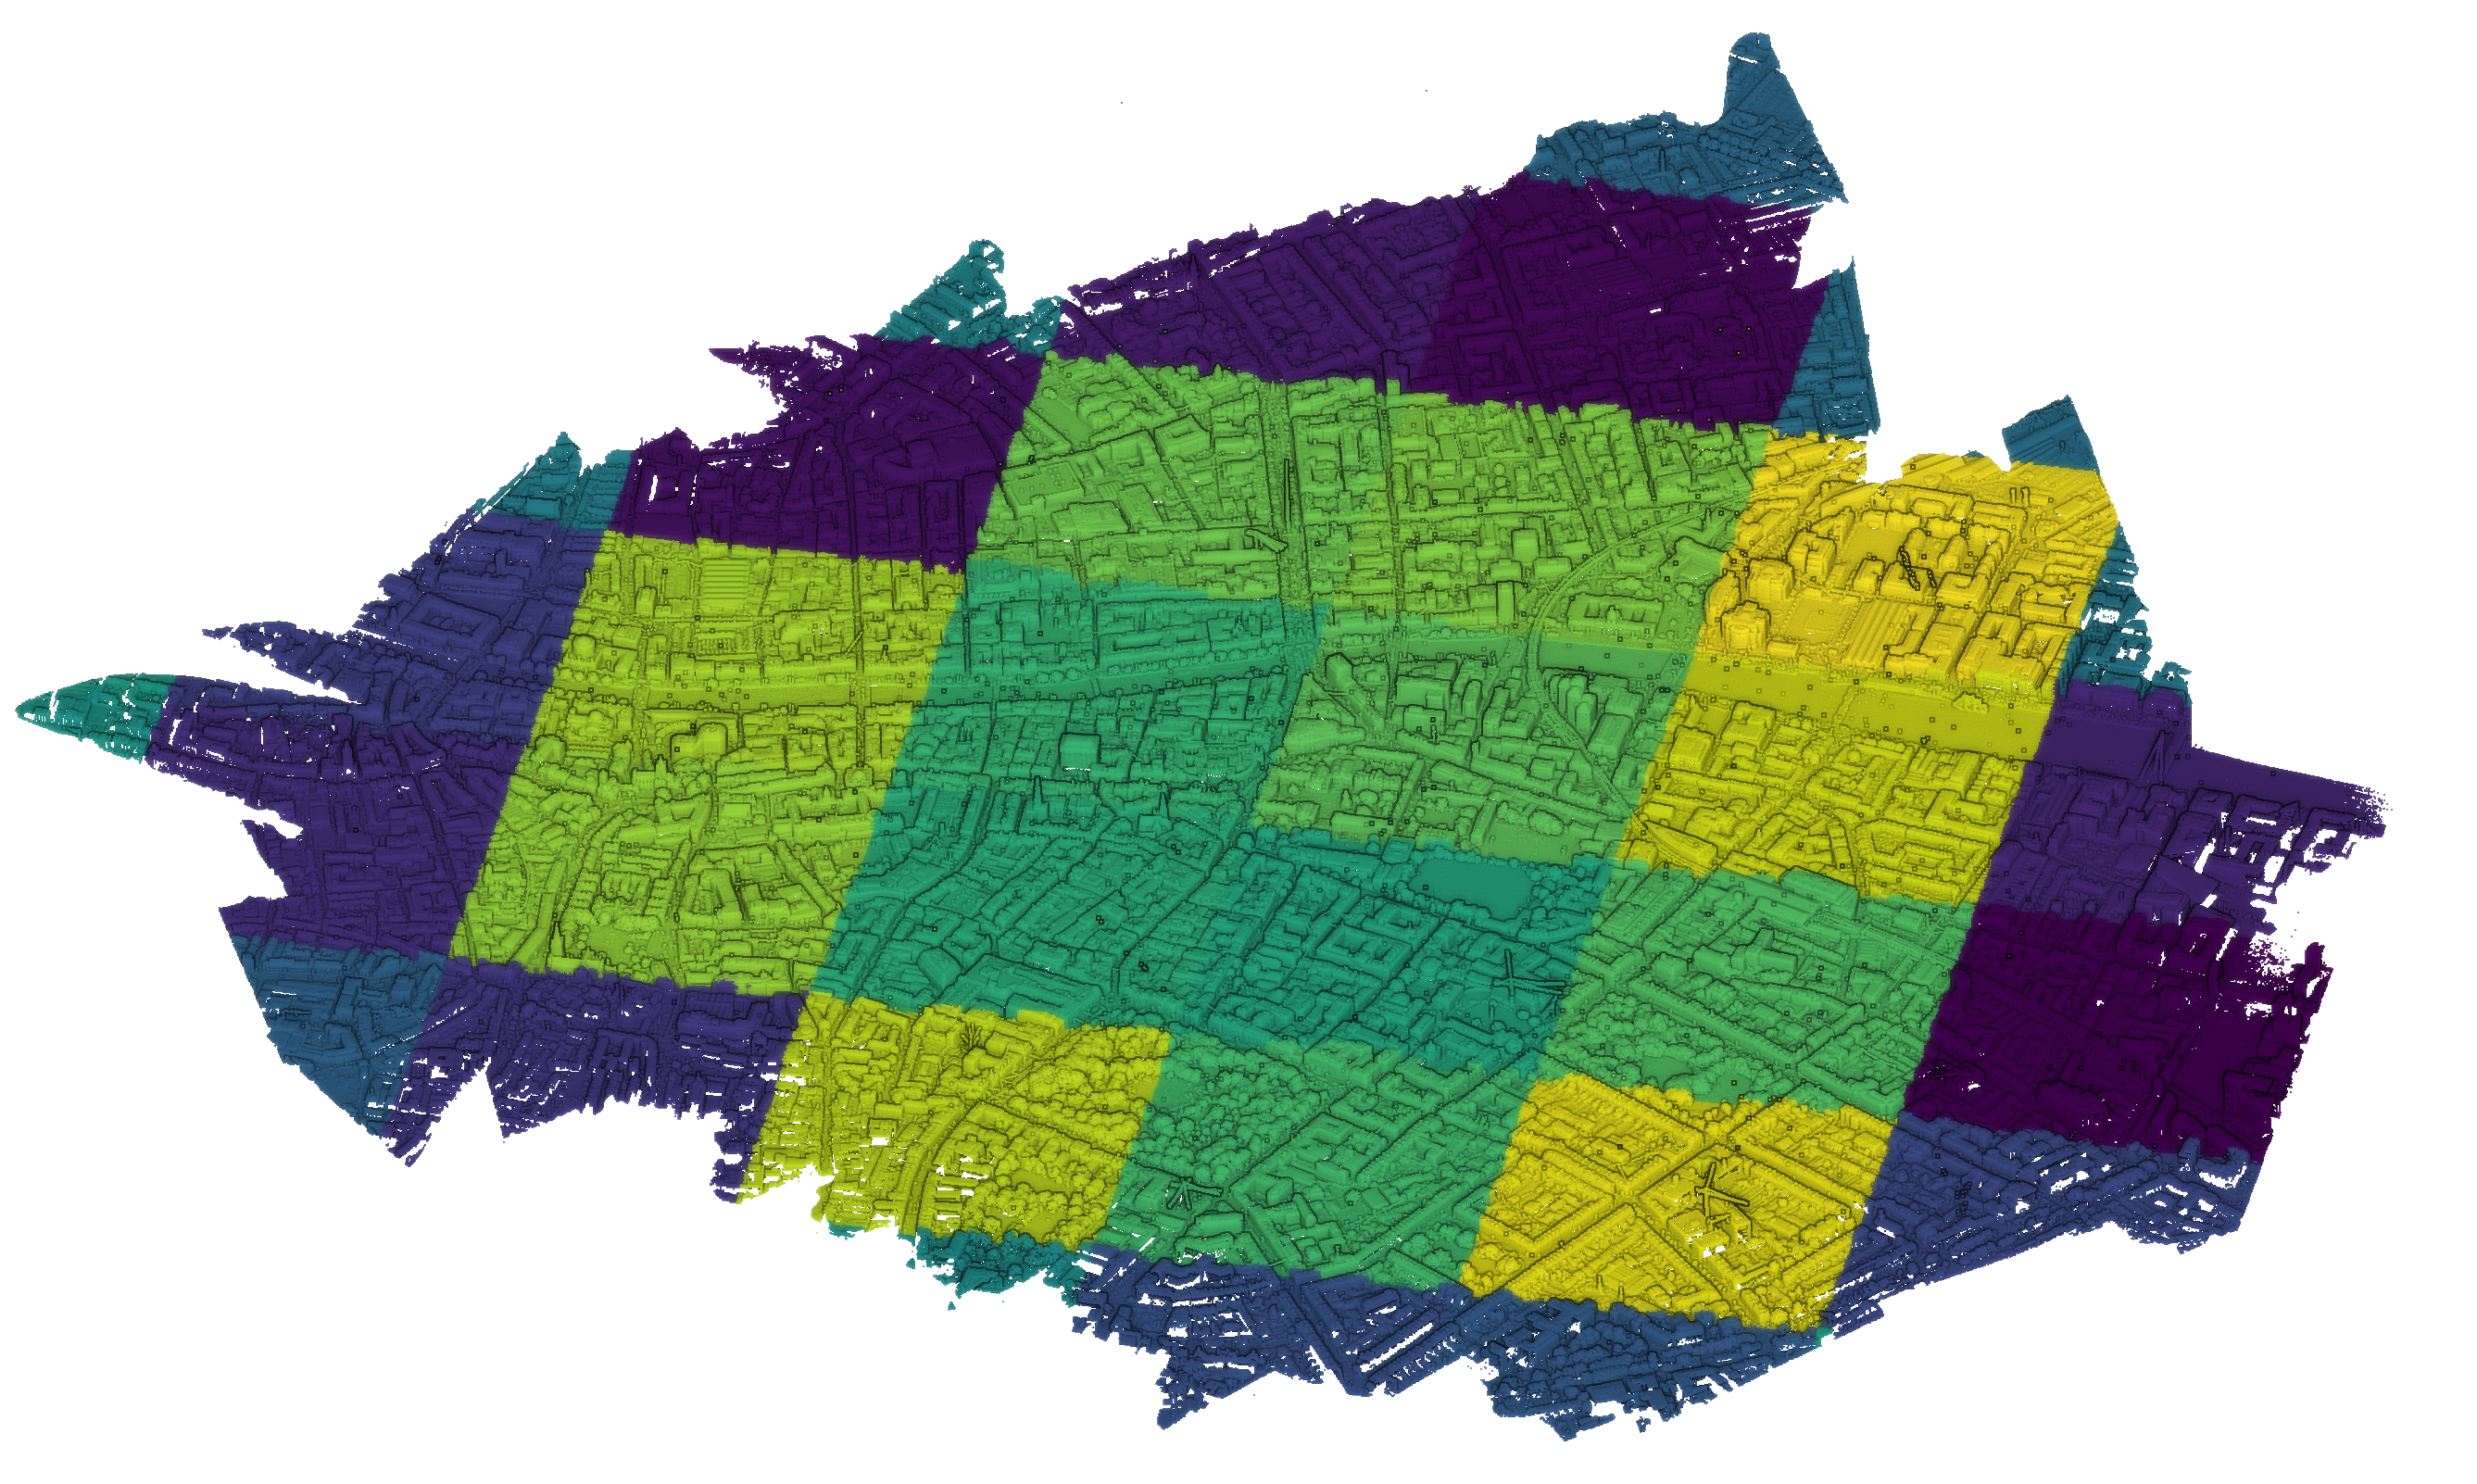
\includegraphics[width=0.45\linewidth]{dublin_parts}
		\includegraphics[width=0.45\linewidth]{terrain_multipart}
	\end{center}
\end{frame}



\bibliographystyle{alphaurl}
\bibliography{bibliography}

\end{document}